%%%%%%%%%%%%%%%%%%%%%%%%%%%%%%%%%%%%%%%%%%%%%%%%%%%%%%%
%%% LATEX FORMATTING - LEAVE AS IS %%%%%%%%%%%%%%%%%%%%
\documentclass[11pt]{article} % documenttype: article
\usepackage[top=20mm,left=20mm,right=20mm,bottom=15mm,headsep=15pt,footskip=15pt,a4paper]{geometry} % customize margins
\usepackage{times} % fonttype
\usepackage{listings}
\usepackage{graphicx}
\usepackage{subcaption}
\graphicspath{ {../images/} }
\makeatletter         
\def\@maketitle{   % custom maketitle 
\begin{center}
{\bfseries \@title}
{\bfseries \@author}
\end{center}
\smallskip \hrule \bigskip }

\mathchardef\mhyphen="2D

%%%%%%%%%%%%%%%%%%%%%%%%%%%%%%%%%%%%%%%%%%%%%%%%%%%%%%%%%%%%%%%%%%%%
%%% MAKE CHANGES HERE %%%%%%%%%%%%%%%%%%%%%%%%%%%%%%%%%%%%%%%%%%%%%%
\title{{\LARGE Information Retrivel: Lab 2}\\[1.5mm]} % Replace 'X' by number of Assignment
\author{Shifei Chen} % Replace 'Firstname Lastname' by your name.

%%%%%%%%%%%%%%%%%%%%%%%%%%%%%%%%%%%%%%%%%%%%%%%%%%%%%%%%%%%%%%%%%%%%
%%% BEGIN DOCUMENT %%%%%%%%%%%%%%%%%%%%%%%%%%%%%%%%%%%%%%%%%%%%%%%%%
%%% From here on, edit document. Use sections, subsections, etc.
%%% to structure your answers.
\begin{document}
\maketitle

\section{Query Experiments}

I'm focusing on the \verb|Glasgow Herald 95| data set and my selected relevance accessment file is \\
\verb|AH-ENGLISH-CLEF2006.txt|.

Below are the three topics I've chosen.

\subsection{C311 Unemployment in Europe}

The first query term I've tried is the one from the title ``unemployment rate Europe'', which gave me an map of 0.25 and precision at 0.574. The problem is if we look at the interpolated precision graph, the line started from 0.6 and went down to 0 at 0.6 of recall.

To raise the precision, The first thing I've tried was to expand the term ``Europe'' to a wide range of synonyms consisiting of some European countries. That increased the initial precison to 1, which means the user should see more  relevant documents from the first few results.

Then I continued to expand other words to their synonyms including ``company'', ``job'', ``figure'', etc, connected with the belief operator \verb|#or()| since we were using these words to classifier documents related to the employment topic. These words don't have to all be present in the same document. As a result, the precision line continued to be more smooth. However one thing doesn't work well is the word window feature. Things like \verb|\#1(employment rate)| dropped the overall map siginificantly. I believe the reason behind that is perhaps it limited the keyword term to be strictly ordered word pairs ``(employment rate)'', which might be too specific.

My final query term is

\begin{lstlisting}
    #combine(
        {unemployment employment}
        {rate figure number percentage}
        {Europe EU Germany Britain UK England France Spain}
        #or(
            {company employer}
            {job work labour}
            {employment hire work}
            {employee worker #1({white blue} collar)}
        )
    )
\end{lstlisting}

The highest map was 0.30 and the over all precision was 0.556. The numbers didn't improve a lot but the interpolated precision line was much somoother than my first attempt.

\begin{figure}[p]
    \centering
    \begin{subfigure}{0.45\textwidth}
      \includegraphics[width=0.9\linewidth]{311/figure_1.png}
      \caption{Original}
    \end{subfigure}
    \begin{subfigure}{0.45\textwidth}
        \includegraphics[width=0.9\linewidth]{311/figure_2.png}
        \caption{After Expanding ``Europe''}
    \end{subfigure}
    \begin{subfigure}{0.45\textwidth}
        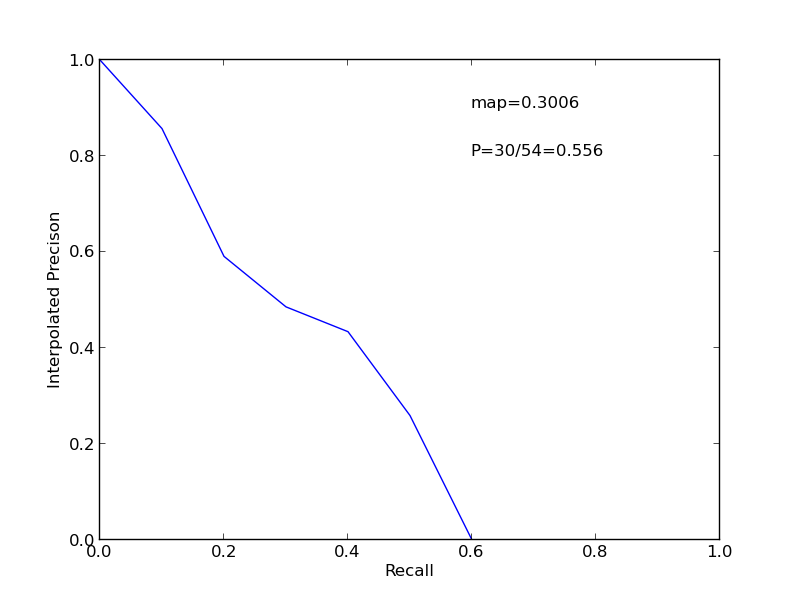
\includegraphics[width=0.9\linewidth]{311/figure_3.png}
        \caption{``Final''}
    \end{subfigure}
    \caption{Interpolated Precisions for Topic C311}
\end{figure}

\subsection{C342 Four Weddings and a Funeral}

In this topic I tried \verb|#weight()| operator instead of \verb|#combine()|. As the title suggests we were looking for the movie so I've put the movie title inside \verb|#1()| to search the title as a whole word.

Later in the description of the topic it mentioned that we should focus on the documents talking about its popularity instead of plot, hence I've given a higher weight to words like ``success'', ``popular'', etc and lower other movie related words such as ``film'', ``movie'', ``theater''.

Below you can see the result of given equal weights to all search terms and ranked weights to them. The ranked weight query term was

\begin{lstlisting}
    #weight(
        1.0 #weight(
            1.0 #1(Four Weddings and a Funeral)
            0.7 {success successful hit popularity popular}
            0.7 {critic response react reaction love hate}
        )
        0.2 {film movie comedy}
        0.1 {cinema theater tickets}
    )
\end{lstlisting}

which results in $map=0.2526, P=0.334$. The map score was higher than the equal weighed query by 0.009.

\begin{figure}[p]
    \centering
    \begin{subfigure}{0.45\textwidth}
      \includegraphics[width=0.9\linewidth]{342/figure_1.png}
      \caption{Without \#weight()}
    \end{subfigure}
    \begin{subfigure}{0.45\textwidth}
        \includegraphics[width=0.9\linewidth]{342/figure_2.png}
        \caption{With \#weight()}
    \end{subfigure}
    \caption{Interpolated Precisions for Topic C311}
\end{figure}

\subsection{C350 Ayrton Senna's Death}

Some of the topics are not easy to retrieve. For example in topic \verb|C350| we need to find out docuemnts related to Ayrton Senna's death, so I tried to search with query \verb|#1(Ayrton Senna)|. Of all the 28 documents returned from the query, none of them are relevant. Then I added synonyms \verb|{#1(Ayrton Senna) Senna}| to search docuemnts which only contains his last name but still none of the docuemtns were relevant. Ayrton Senna's name is the same in Portuguese and English so it can't be the problem of spelling. I doubt if it was possible to write a document about his death without mentioning his name.

I also tried other keywords like ``Imola''(where the accident was happened) but still the results were the same. Also this happened to other topics such as \verb|C333| where I searched both ``Paul Touvier'' and ``Touvier'' and all 3 returned documents were not in the 5 relevant document set. In topic \verb|C301| the description clearly stated that the brand name ``Nestlé'' should be in the document, but only 3 docuemnts from the query result were actually relevant where there were other 13 relevant documents which didn't contain the name of the brand.

\section{Automated Query}

To save the effort of creating the query parameter xml files and running other command line tools, I have written a python script to speed things up. To run the code you need to provide a JSON configuration file, in which you point to the location of your query index selected qrel file.

After that you can run the script like

\begin{lstlisting}
    python3 query.py 350 "{#1(Ayrton Senna) Senna}"
\end{lstlisting}

The first parameter is the id of that topic, the second one is a string representation of your query term.

There's also some help messages by running \verb|python3 query.py -h|.

\end{document}